\chapter{Solving Systems of Linear Equations}



\section{Solving Triangular Systems}
We will begin our solution of general linear equations by considering how to solve triangular systems.  This simpler form of system is particularly easy to solve, and it is easy to make other systems become triangular.  In later sections reducing a matrix to triangular form becomes a standard tool.

As a side note, we really don't like reducing to a triangular matrix.  It is better to reduce to upper or lower Hessenberg form\footnote{triangular plus one non-zero diagonal immediately past the main diagonal}.  Similarly, real numerical systems often avoid diagonalizing and reduce to tridiagonal matrix\footnote{The only non-zero elements are on the main diagonal and the diagonals immediately next to it}.  The reason is it is often difficult to zero the elements right next to the main diagonal, so we often get most of the way and then finish the job with an iterative method.  Starting with an iterative method would be slow.  This way we get the best of both systems.

\subsection{Forward Substitution}

Consider a system $Lx=b$, where $L$ is a square lower triangular matrix.
\begin{eqnarray}
\left[\begin{matrix}
l_{1,1} & 0       & \cdots & 0 \\
l_{2,1} & l_{2,2} & \ddots & \vdots \\
\vdots  & \vdots  & \ddots & 0 \\
l_{n,1} & l_{n,2} & \cdots & l_{n,n}
\end{matrix}\right]
\left[\begin{matrix}
x_1 \\
x_2 \\
\vdots \\
x_n
\end{matrix}\right]
&=&
\left[\begin{matrix}
b_1 \\
b_2 \\
\vdots \\
b_n
\end{matrix}\right] \label{eq-lowertriangluarLS}
\end{eqnarray}
The first row tells us
\begin{eqnarray}
l_{1,1}x_1 &=& b_1 \nonumber \\
x_1 &=& \frac{b_1}{l_{1,1}} \label{eq-lowertriangluarLS-row1}
\end{eqnarray}
Using the solution of the first line and the equation of the second row we find
\begin{eqnarray}
l_{2,1}x_1 + l_{2,2}x_2 &=& b_2 \nonumber \\
x_2 &=& \frac{b_2-l_{2,1}x_1}{l_{2,2}} \\
x_2 &=& \frac{b_2-l_{2,1}\frac{b_1}{l_{1,1}}}{l_{2,2}} \nonumber
\end{eqnarray}
In essence we are removing the effect of $x_1$ on $b$ and then solving just as we did in Eq~\ref{eq-lowertriangluarLS-row1}.  With the knowledge of $x_2$ we will need to remove its effect on $b$ for subsequent calculations.  We can generalize this into a simple procedure.  The one thing we have to make sure is that the elements on the main diagonal never become zero\footnote{There are a lot of ways of explaining why this is from the matrix itself, here are a two.  For lower (or upper) triangular systems the determinant is the product of the diagonal elements, thus if one is zero then the determinant is zero and no inverse exists.  A zero on the diagonal of a triangular (upper or lower) matrix means there is a zero eigenvalue, and hence the matrix is not invertible.}, as we need to divide by them.
\SciLab{SciLab code for forward substitution}{cod-forward-substitution}{scilab/forward_substitution.sci}
Listing~\ref{cod-forward-substitution} shows SciLab code for a forward substitution function.  Note that it has complexity $\frac{n^2}{2}$, which is much better than the $n^3$ for matrix inversion.  In Listing~\ref{cod-forward-substitution-test}, is SciLab code that uses the forward substitution function.  The exec command causes SciLab to run the contents of the file containing forward\_substitution, thus defining it for use on the next line.
\SciLab{SciLab test code for forward substitution}{cod-forward-substitution-test}{scilab/forward_substitution_test.sce}

\subsection{Backward Substitution}

Now consider a system $Ux=b$, where $U$ is a square upper triangular matrix.
\begin{eqnarray}
\left[\begin{matrix}
u_{1,1} & u_{1,2} & \cdots & u_{1,n} \\
0       & u_{2,2} & \cdots & u_{2,n} \\
\vdots  & \ddots  & \ddots & \vdots \\
0       & \cdots  & 0      & u_{n,n}
\end{matrix}\right]
\left[\begin{matrix}
x_1 \\
x_2 \\
\vdots \\
x_n
\end{matrix}\right]
&=&
\left[\begin{matrix}
b_1 \\
b_2 \\
\vdots \\
b_n
\end{matrix}\right] \label{eq-uppertriangluarLS}
\end{eqnarray}
The last row tells us
\begin{eqnarray}
u_{n,n}x_n &=& b_n \nonumber \\
x_n &=& \frac{b_n}{u_{n,n}} \label{eq-uppertriangluarLS-row1}
\end{eqnarray}
Using the solution of the last line and the equation of the second to last row we find
\begin{eqnarray}
u_{n-1,n}x_n + u_{n-1,n-1}x_{n-1} &=& b_{n-1} \nonumber \\
x_{n-1} &=& \frac{b_{n-1}-u_{n-1,n}x_n}{u_{n-1,n-1}} \\
x_{n-1} &=& \frac{b_{n-1}-u_{n-1,n}\frac{b_n}{u_{n,n}}}{u_{n-1,n-1}} \nonumber
\end{eqnarray}
In essence we are removing the effect of $x_n$ on $b$ and then solving just as we did in Eq~\ref{eq-uppertriangluarLS-row1}.  With the knowledge of $x_{n-1}$ we will need to remove its effect on $b$ for subsequent calculations.  We can generalize this into a simple procedure.  As in the lower triangular matrix of the forward substitution case, the one thing we have to make sure is that the elements on the main diagonal never become zero\footnote{There are a lot of ways of explaining why this is from the matrix itself, here are a two.  For lower (or upper) triangular systems the determinant is the product of the diagonal elements, thus if one is zero then the determinant is zero and no inverse exists.  A zero on the diagonal of a triangular (upper or lower) matrix means there is a zero eigenvalue, and hence the matrix is not invertible.}, as we need to divide by them.
\SciLab{SciLab code for backward substitution}{cod-backward-substitution}{scilab/backward_substitution.sci}
Listing~\ref{cod-backward-substitution} shows SciLab code for a backward substitution function.  Note that it has complexity $\frac{n^2}{2}$, which is much better than the $n^3$ for matrix inversion.  In Listing~\ref{cod-backward-substitution-test}, is SciLab code that uses the backward substitution function.  The exec command causes SciLab to run the contents of the file containing backward\_substitution, thus defining it for use on the next line.
\SciLab{SciLab test code for backward substitution}{cod-backward-substitution-test}{scilab/backward_substitution_test.sce}

\section{LU Factorization}

Since we have ways to solve a system of matrices, $Ax=b$, where $A$ is either upper or lower triangular, it makes sense to ask can we transform any matrix into this form and then solve it.  It turns out we can, and it is fairly fast, but not numerically stable\footnote{Basically this means it can give very wrong answers under certain circumstances.  Don't do this with badly conditioned matrices unless you really know what you are doing.}.  First I provide code in Listing~\ref{cod-lu_no_pivot} to find both $L$ (a lower triangular matrix) and $U$ (an upper triangular matrix), such that $LU=A$.  Theoretically you could use this and your forward and backward solver to get the solution.  In practice we don't do this for two reasons.  First, it cannot handle a zero value on the main diagonal (row $=$ col), which will be handled by pivoting.  Second, though is that we don't need to know $L$, we just need $U$ and $L^{-1}b$.  This can be seen by the following
\begin{eqnarray}
Ax &=& b \\
LUx &=& b
\end{eqnarray}
Note that this step is seen simply by noting $A=LU$ by construction of $L$ and $U$.
\begin{eqnarray}
LUx &=& b \\
L^{-1}LUx &=& L^{-1}b \\
Ux &=& L^{-1}b
\end{eqnarray}
The next step is the basic algebraic rule of multiplying both sides by the same thing does not change them.  The last step combines the definition of an inverse, namely $L^{-1}L=I$, and the property of $I$ that $IU=U$.  Thus to find $x$ we need $U$ and $L^{-1}b$.  The code for this is in Listing~\ref{cod-lusolver_no_pivot}.  Note you could also just write a function that returns $U$ given $A$, and then pass $\left[\begin{matrix}A & b\end{matrix}\right]$ instead of just $A$, and your function will return $\left[\begin{matrix}U & L^{-1}b\end{matrix}\right]$.

\SciLab{Gaussian Elimination (LU factorization)}{cod-lu_no_pivot}{scilab/lu_no_pivot.sci}
\SciLab{Solving $Ax=b$ using LU factorization}{cod-lusolver_no_pivot}{scilab/lusolver_no_pivot.sci}

\subsection{Partial Pivoting}

\SciLab{Gaussian Elimination with row pivoting (LU factorization with partial pivoting)}{cod-lu_partial_pivot}{scilab/lu_partial_pivot.sci}

\subsection{Cholesky Factorization}

For symmetric ($A=A^T$), positive definite ($x^TAx>0\;\forall x\neq 0$) we can perform a special form of the LU factorization called the Cholesky factorization ($A=LL^T$).  To see how this works consider the following
\begin{eqnarray*}
L &=& \left[\begin{matrix}
l_{1,1} & 0       & \cdots & 0 \\
l_{2,1} & l_{2,2} & \ddots & \vdots \\
\vdots  & \vdots  & \ddots & 0 \\
l_{n,1} & l_{n,2} & \cdots & l_{n,n}
\end{matrix}\right] \\
LL^T &=&\left[\begin{matrix}
l_{1,1} & 0       & \cdots & 0 \\
l_{2,1} & l_{2,2} & \ddots & \vdots \\
\vdots  & \vdots  & \ddots & 0 \\
l_{n,1} & l_{n,2} & \cdots & l_{n,n}
\end{matrix}\right]\left[\begin{matrix}
l_{1,1} & l_{2,1} & \cdots & l_{n,1} \\
0       & l_{2,2} & \cdots & l_{n,2} \\
\vdots  & \ddots  & \ddots & \vdots \\
0       & \cdots  & 0      & l_{n,n}
\end{matrix}\right] \\
&=& \left[\begin{matrix}
l_{1,1}^2      & l_{1,1}l_{2,1}      & \cdots & l_{1,1}l_{n,1} \\
l_{2,1}l_{1,1} & l_{2,2}^2+l_{2,1}^2 & \ddots & \vdots \\
\vdots         & \ddots              & \ddots & l_{n,n-1}l_{n-1,n-1}+\sum_{i=1}^{n-2}l_{n,i}l_{i,n-1} \\
l_{n,1}l_{1,1} & \cdots              & l_{n,n-1}l_{n-1,n-1}+\sum_{i=1}^{n-2}l_{n,i}l_{i,n-1} & l_{n,n}^2+\sum_{i=1}^{n-1}l_{n,i}^2
\end{matrix}\right]
\end{eqnarray*}


\SciLab{Cholesky Factorization}{cod-cholesky}{scilab/Cholesky.sci}

\section{QR Factorization}

While in most practical systems LU or a specialized version like Cholesky will work nicely, there are times when numerical conditioning makes these methods dangerous.  This is when we can use a more numerically savvy routine, QR factorization.  The idea of QR factorization is to obtain an upper triangular matrix, $R$, similar to LU, but to do it with orthogonal transformations. Orthogonal transforms use orthogonal matrices, which have a variety of nice properties
\begin{enumerate}
  \item The inverse is the transpose ($Q^{-1}=Q^T$)
  \item The norm is 1 ($\|Q\|=1$)
  \item The norm of the inverse is 1 ($\|Q^{-1}\|=\|Q^T\|=\|Q\|=1$)
  \item The condition number is 1 ($cond(Q)=\|Q\|\|Q^{-1}\|=1$)
\end{enumerate}
The first and last property are particulary nice for us.  Since the condition number is 1, we should not cause any errors to grow.  Since the transpose is the inverse it is easy and relatively quick to calculate.  There are several ways to do QR, which revolve around how to form $Q$ or $R$.  To understand these methods, you first need to understand basis, dimensionality of vector spaces, and orthogonality, but those in turn requires an understanding of independence.  If you are not familiar with any of these concepts please read Section~\ref{s-basis}.

\subsection{Gram-Schmidt Orthogonalization}
This is the easiest to understand, but the worst to do.
\SciLab{Classic Gram-Schmidt Orthogonalization}{cod-gramschmidt_classic}{scilab/gram_schmidt_classic.sci}

\subsection{Modified Gram-Schmidt Orthogonalization}
The fix gains some precision but does not fix the root problem.
\SciLab{Modified Gram-Schmidt Orthogonalization}{cod-gramschmidt_modified}{scilab/gram_schmidt_modified.sci}

\subsection{Givens Rotations}
This works well, and is best suited to sparse matrix solvers because it can be used to target individual, non-zero elements without effecting other terms.  Each Givens rotation only effects only two rows or columns in the target matrix (depends on if you do left or right multiplication). A rotation matrix is given by
\begin{eqnarray}
R_{\theta} &=& \left[\begin{matrix}\cos\theta & -\sin\theta\\
                                   \sin\theta & \cos\theta\end{matrix}\right].
\end{eqnarray}
Givens rotations are the 4 elements of a rotation matrix in a square pattern centered on the diagonal.  Being rotations they are very nice to calculate, easy to express, but have a higher overhead to do them for every non-zero term.  When there are only a few non-zero terms (i.e. sparse matrices) this is not bad, and they end up being much more efficient than other methods that will calculate how to zero a zero element.

\subsection{Householder Reflections}
This works well, and is best suited to dense matrix solvers.  When matrices have mostly non-zero elements (i.e. ``dense matrices'') the low overhead of zeroing an entire column with a Householder reflector is very efficient.  These are hyperbolic, since they are reflectors, so they can have some calculation problems, though this is not common.  First I will state the result then I will prove it.
\begin{eqnarray}
H_i &=& I-2vv^T \\
u&=& a_i(i:m)-e_1\|a_i(i:m)\|\\
v&=& \frac{u}{\|u\|}
\end{eqnarray}
Note that by our construction that $v^Tv = 1$.  Additionally, observe that the size of the matrix diminishes by one row and column each iteration, this is because once a column has been reduced, one more row does not need to be effected.  Due to this we only need to work on $A(i:m,i:n)$.

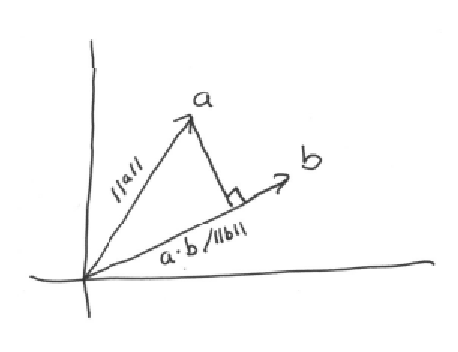
\includegraphics{projection.eps}

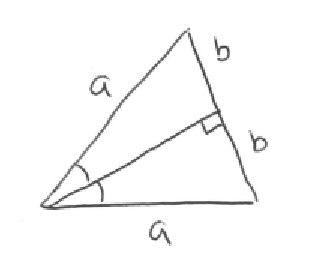
\includegraphics{isosoles_triangle.eps}

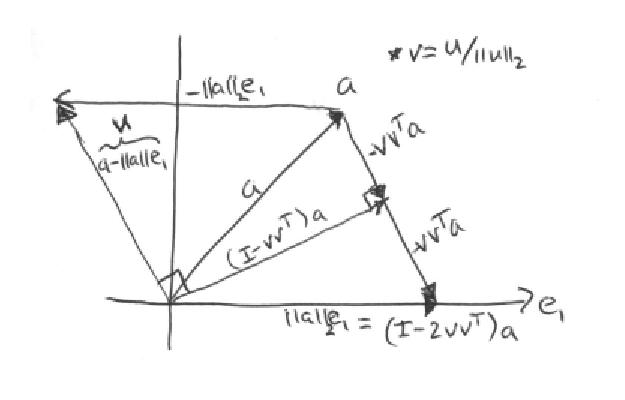
\includegraphics{householder.eps}


\section{Singular Value Decomposition}

The SVD is extremely stable and is in some sense the ultimate safe thing to do, if it is done right anyway.  We do not often do it as it is expensive (read slow) to calculate.  The danger in QR is in error buildup in solving, $R$, by back substitution.  It would be much nicer to have a diagonal matrix so errors couldn't buildup.  The SVD always exists and is a non-unique (i.e. there are many different SVD's for the same matrix) decomposition that is given by
\begin{eqnarray}
A &=& U\Sigma V^T
\end{eqnarray}
where $U$ and $V$ are unitary (generalization of orthogonal to complex numbers) matrices, and $\Sigma$ is  a diagonal matrix with the main diagonal ordered so $\sigma_1\geq\sigma_2\geq\cdots\geq\sigma_n\geq 0$.  Thus $\Sigma$ is not only diagonal, it is positive semidefinite (there could be zeros on the diagonal) and ordered.  We can even calculate individual singular values (the $\sigma_i$).  Some popular uses are
\begin{enumerate}
\item $\|A\|_2=\sigma_1$
\item $\|A^{-1}\|_2=\sigma_n^{-1}$
\item $cond(A)=\frac{\sigma_1}{\sigma_n}$
\item $\|A\|_{Frobenius}^2=\sum_{i=1}^n\sigma_i^2$
\item $A^{-1} = V\Sigma^{-1}U^T$, note $\Sigma^{-1}$ is easy to calculate because it is diagonal.
\end{enumerate} 